\section{DUNE Computing Model}
\label{sec:computing_model}

\subsection{Summary of data rate and volume estimates}
Rate and volume of the data to be produced by DUNE detector systems are the major driver determining the parameters
of the DUNE computing model. These characteristics  have been presented and discussed in Sec.~\ref{sec:fd-data-overview}.

At the time of writing estimations for the Far Detector data are the best understood, due to better defined geometry,
technology and configuration choices, and considerations presented in subsections~\ref{sec:daq-assumptions},~\ref{sec:zs-data}
and \ref{sec:data-compression}.

A distinguishing characteristic of the data flow in DUNE Far Detector is an enormous data reduction factor to be achieved
in the Far Detector DAQ, as evidenced by the numbers presented in Tables~\ref{tab:full-stream-volume} and \ref{tab:zs-volume}.
The key assumption in this is the capability of DAQ to distinguish low energy signals  due to $^{39}$Ar decays spread
across the volume of the detector from more interesting physics phenomena. Estimates of volume of data due to
high-energy interaction (cosmic $\mu$ and beam neutrinos) are presented in Table~\ref{tab:fd-data-volume-summary}
and are quite modest.

Processing required to identify candidate SNB and nucleon decay events will also be handled by the online systems.
As discussed in subsection \ref{sec:snb-data}, once a SNB trigger condition has been established, the data must
be recorded without zero suppression in order to capture the characteristically low energy and scattered ionization
clusters in the detector volume. As shown in Table~ \ref{tab:zs-volume}, the resulting volume of data is significant
and is currently estimated as just over half a PB annually, given the premise of accepting roughly 12 false positives per year.
While the main goal of the SNB trigger is to provide a close to real-time Supernova Burst alert, the data flagged by DAQ
as candidate should not be discarded as it can be used to better understand and improve online algorithms.

%Identifying candidate nucleon decay events will also require sophisticated algorithms and 

Thee Near Detector data estimates are very preliminary (see~\ref{sec:nds-event-rates}) and result in annual
volume from a few dozen to a hundred TB.

In summary, it is anticipated that under assumptions presented above the total volume of data in DUNE to be
committed to storage will be up to 1PB per year of data taking.

\subsection{Far Detector Data Management}
\subsubsection{The Big Picture}
A high-level conceptual diagram of the data flow in DUNE in presented in Fig.\ref{fig:DUNEdataflow}.
The top section of the diagram (labeled ``A'') represents systems and data flow at the Far Site.
The mid-section ``B'' depicts the DUNE data storage network. FNAL is the main data center
hosting tape storage for the primary copy of all data, as well as distributed disk (such as dCache).
It is expected that the Metadata system will also be deployed and operated at FNAL.
Additional Grid sites at participating institutions will have replicas of the data.
Replication of the data will be done as per requirements formulated in \ref{sec:req-raw-data-replication}.

\begin{figure}[h!]
\centering
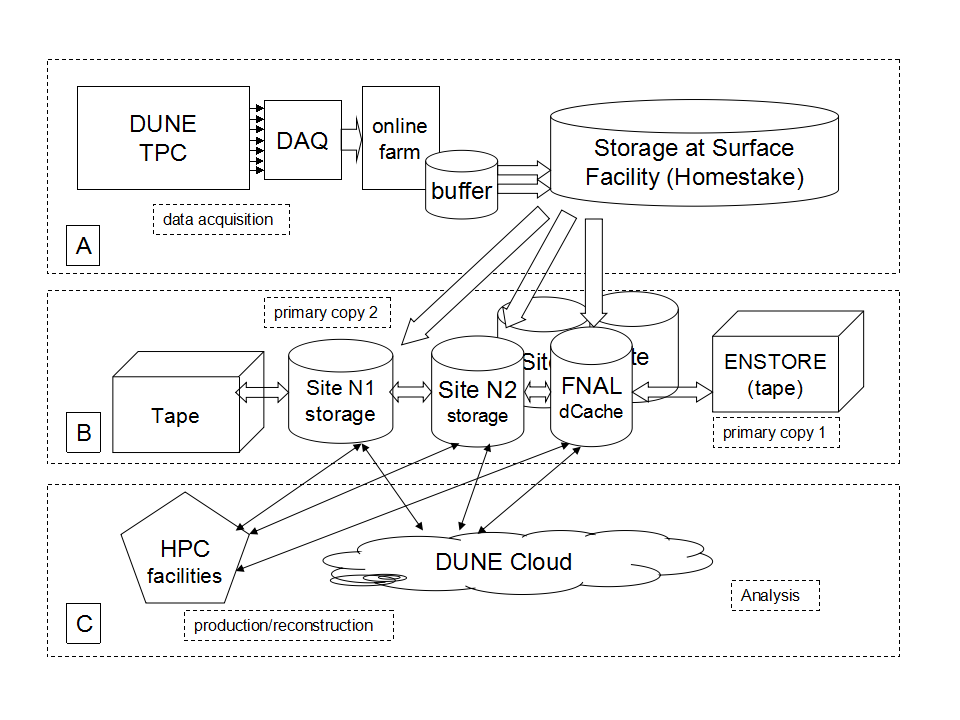
\includegraphics[width=\textwidth]{DUNEdataflow.png}
\caption{Conceptual Diagram of the Data Flow in DUNE.}
\label{fig:DUNEdataflow}
\end{figure}

\subsubsection{Data Handling at the Far Site}
Data Acquisition systems will be located in the specially built rooms in the detector vicinity, i.e. deep in the cavern (commonly referred to as 4850L).
The undergound location is to be connected to surface by 96-strand fiber optic cable, but this does not imply that all strands will be
utilized at any given time. The scale of bandwidth of an individual fiber is 10gbps. It can be therefore expected that there will be ample headroom
for data transmission to the surface under a variety of scenarios.

There will be two layers of data buffering: a buffer in DAQ before the data is transmitted to the surface,
and at the surface facility before the data is transmitted to FNAL which is the primary storage site and the
keeper of the custodial copy of the data. It is a common practice to provide buffer space for the experiment
which is sufficient for intermediate storage of data for one or a few days in order to keep running even in case
of network equipment outages. Given the estimates presented above, the decisive factor for determining the buffer
size will be the data scale of candidate SNB events since they are likely to be read out at full-stream rate (with lax or
no zero-suppression) (see Table~\ref{tab:zs-volume}). The size of each buffer (the online farm and the surface facility
as drawn in section ``A'' of Fig.\ref{fig:DUNEdataflow}) can therefore be estimated as $\sim$50\,TB.

 There are additional considerations due to the modular structure of the DUNE Far Detector
which is conceived as four individual TPC modules. In order to minimize down time and the number of potential single points of failure,
DAQ will be segmented into four individual  systems each collecting data from a respective module. To ensure
consistency and simplicity of processing, it is desirable to merge the resulting data streams coming from individual detectors at some point
so that data is written to files each containing data for the full 4-module DUNE detector. The surface facility is the optimal location
for the merging to take place since it needs to be equipped with storage for buffering purposes in any event.

\subsubsection{Data Handling at the Near Site}
\fxnote{Just a placeholder at this point}
The Near Site is located within the boundaries of Fermilab and therefore it is easier to provide networking and other services for data handling.


